%%%%%%%%%%%%%%%%%%%%%%%%%%%%%%%%%%%%%%%%%%%%%%%%%%%
\begin{frame}
  \begin{center}
    {\Large RNN with TensorFlow}
    
  \end{center}
\end{frame}


%%%%%%%%%%%%%%%%%%%%%%%%%%%%%%%%%%%%%%%%%%%%%%%%%%%
\begin{frame}[fragile] \frametitle{Predicting Google Stock Price}
\begin{itemize}
\item Dataset: Google Stock prices, 2012 to 2016.
\item LSTM to cpature upward or downward trend, predict Jan 2017 trend.
\item Better than traditional ARIMA model
\end{itemize}
(Ref: Deep Learning A-Z - Kirill Eremenko https://www.udemy.com/deeplearning/learn/v4/t/lecture/8374794)
\end{frame}



%%%%%%%%%%%%%%%%%%%%%%%%%%%%%%%%%%%%%%%%%%%%%%%%%%
\begin{frame}[fragile] \frametitle{Predicting Google Stock Price}
Input
\begin{center}
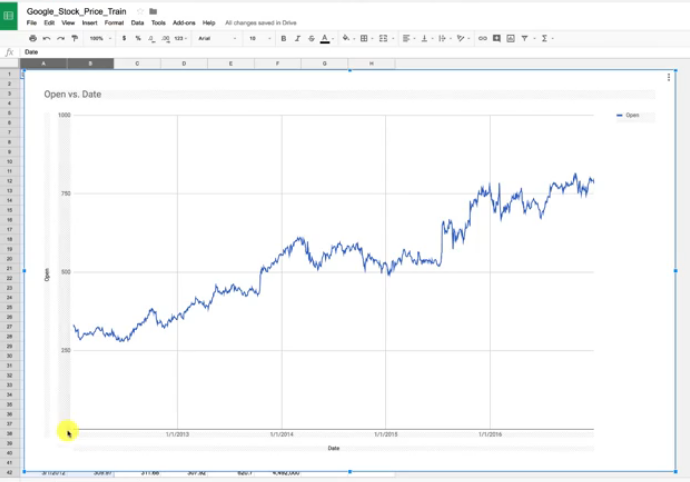
\includegraphics[width=0.7\linewidth,keepaspectratio]{lstm44}
\end{center}
Test set has same columns (there is no target column missing, as such) in Time serries analysis. We are predicting next value. Test set has Jan 2017 values to compare predictions with.
\end{frame}


%%%%%%%%%%%%%%%%%%%%%%%%%%%%%%%%%%%%%%%%%%%%%%%%%%
\begin{frame}[fragile] \frametitle{Imports of libs and data}

\begin{lstlisting}
import numpy as np
import matplotlib.pyplot as plt
import pandas as pd

dataset_train = pd.read_csv("Google_Stock_Price_Train.csv")
training_set = dataset_train.iloc[:,1:2].values
\end{lstlisting}
Creating numpy array (by .values) of a single column ``Open'' prices.
\end{frame}

%%%%%%%%%%%%%%%%%%%%%%%%%%%%%%%%%%%%%%%%%%%%%%%%%%
\begin{frame}[fragile] \frametitle{Feature Scaling}
\begin{itemize}
\item Standardization: $\frac{x - \mu}{\sigma}$
\item Normalization: $\frac{x - min}{max - min}$
\end{itemize}
Using normalization using scikit learns min max scalar class
\begin{lstlisting}
from sklearn.preprocessing import MinMaxScaler

sc = MinMaxScaler(feature_range=(0,1))
training_set_scaled = sc.fit_transform(training_set)
\end{lstlisting}
\end{frame}


%%%%%%%%%%%%%%%%%%%%%%%%%%%%%%%%%%%%%%%%%%%%%%%%%%
\begin{frame}[fragile] \frametitle{Time Steps}
Super critical to introduce right time steps.
\begin{itemize}
\item Say 60, means, LSTM will look at 60 previous values and the current one, to predict the next value.
\item Just 1 timestep is not good as it leads to over fitting.
\item 20 was not good to catupre the trends. 
\item Its like 60 days moving average graph, ie last 2 months.
\item Will define two variables x\_train and y\_train. For each time t:
\item x\_train will have 60 previous values before the current day.
\item y\_train will have the value of the next day.
\end{itemize}
\end{frame}

%%%%%%%%%%%%%%%%%%%%%%%%%%%%%%%%%%%%%%%%%%%%%%%%%%
\begin{frame}[fragile] \frametitle{Time Steps}
\begin{itemize}
\item As we need previous 60 values, we need to start for loop after that.
\item Ends at the last value,training\_set\_scaled.shape[0], ie 1258
\item x\_train has previous (for i = 60, x\_train has 60-60 ie 0 to 60 values and column is just 0th.
\item y\_train has i + 1 th value, but as index starts with 0, it is i
\item Both are lists, make them numpy arrays to be usable later.
\end{itemize}

\begin{lstlisting}
x_train = []
y_train = []
for i in range(60,training_set_scaled.shape[0]):
    x_train.append(training_set_scaled[i-60: i,0])
    y_train.append(training_set_scaled[i,0])
x_train, y_train = np.array(x_train), np.array(y_train)    
\end{lstlisting}
\end{frame}

%%%%%%%%%%%%%%%%%%%%%%%%%%%%%%%%%%%%%%%%%%%%%%%%%%
\begin{frame}[fragile] \frametitle{Predictors}
\begin{itemize}
\item ``Open'' price is just one predictor we have for now.
\item Need to add  dimension using reshape function, to x\_train
\item Thats one sheet for this feature.
\item Any additional dimension will add new sheets in the 3rd dimension.
\item RNN expects 3d shape:number of obersvations or batch size (1258), time steps (60), predictors (1)
\end{itemize}

\begin{lstlisting}
x_train = np.reshape(x_train,(x_train.shape[0],x_train.shape[1],1))
\end{lstlisting}
\end{frame}

%%%%%%%%%%%%%%%%%%%%%%%%%%%%%%%%%%%%%%%%%%%%%%%%%%
\begin{frame}[fragile] \frametitle{Model}
\begin{itemize}
\item Building NN architecture as usual
\item LSTM layer are arguments:
\begin{itemize}
\item number of units: number of neurons/nodes in each LSTM layer. 50 is good. Just 2 or3 wont capture well.
\item return sequence: True if you want to get last value. When you are building last LSTM layer, then its False
\item input shape:  time steps (60), predictors (1), first argument x\_train.shape[0] is taken automatically
\end{itemize}
\item Including dropout to avoid overfitting.
\end{itemize}
\end{frame}



%%%%%%%%%%%%%%%%%%%%%%%%%%%%%%%%%%%%%%%%%%%%%%%%%%
\begin{frame}[fragile] \frametitle{Input units vs Time Steps}
Time steps specify number of inputs in past. Then whats number of input units in the LSTM layer?
\begin{center}
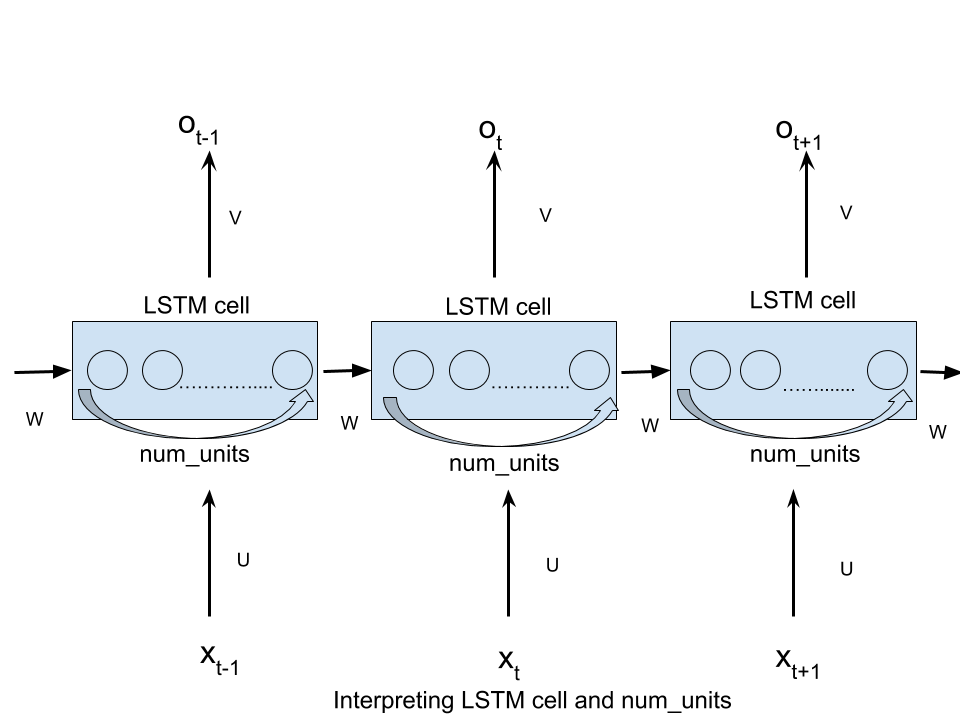
\includegraphics[width=0.5\linewidth,keepaspectratio]{lstm45}
\end{center}
Each blue box is an LSTM layer, composed of multiple cells/units, each of which accepts a vector input x\_t. Each unit cell will take an input of size/units 50. The output size is always 1, similar to neural network nodes (like sigmoidal units) that combine and then activate.
\end{frame}


%%%%%%%%%%%%%%%%%%%%%%%%%%%%%%%%%%%%%%%%%%%%%%%%%%
\begin{frame}[fragile] \frametitle{Code from Scratch}
\begin{center}
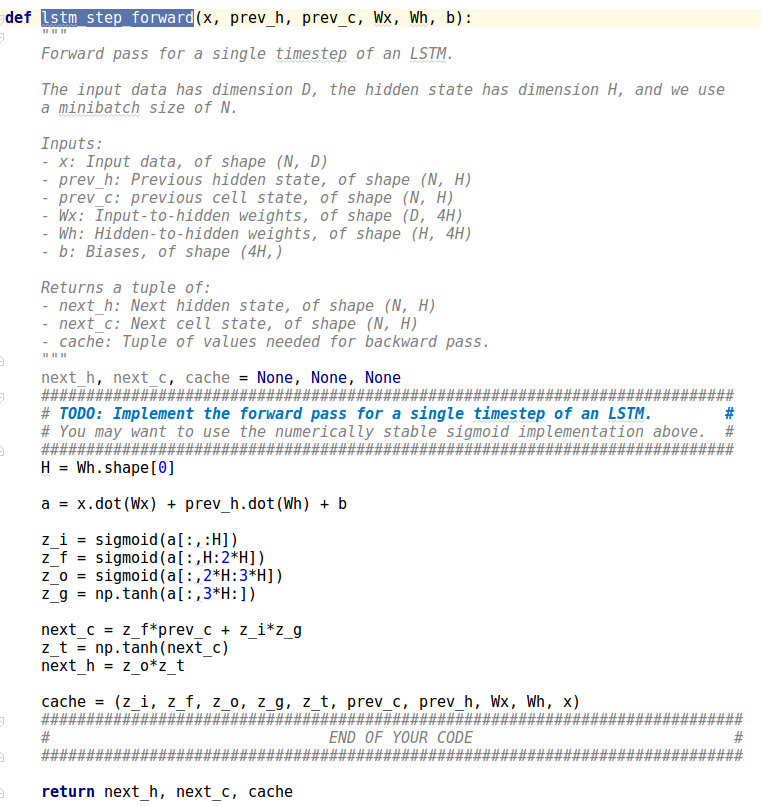
\includegraphics[width=0.6\linewidth,keepaspectratio]{lstm46}
\end{center}
\end{frame}

%%%%%%%%%%%%%%%%%%%%%%%%%%%%%%%%%%%%%%%%%%%%%%%%%%
\begin{frame}[fragile] \frametitle{LSTM Layers}

\begin{lstlisting}
from tf.keras.models import Sequential
from tf.keras.layers import Dense
from tf.keras.layers import LSTM
from tf.keras.layers import Dropout

regressor = Sequential()
regressor.add(LSTM(units=50, return_sequences = True, input_shape = (x_train.shape[1],1)))
regressor.add(Dropout(0.2))
regressor.add(LSTM(units=50, return_sequences = True))
regressor.add(Dropout(0.2))
regressor.add(LSTM(units=50, return_sequences = True))
regressor.add(Dropout(0.2))
regressor.add(LSTM(units=50, return_sequences = False))
regressor.add(Dropout(0.2))
\end{lstlisting}
2nd layer onwards, no need to specify input\_shape. You may keep/change the number of units. Last LSTM has return sequenes to False.
\end{frame}


%%%%%%%%%%%%%%%%%%%%%%%%%%%%%%%%%%%%%%%%%%%%%%%%%%
\begin{frame}[fragile] \frametitle{Output Layer and compiling, fitting}
Adding fully connected layer ie Dense layer.
Output is the stock prediction, which is dimension 1, so outout layer's dim is 1.
\begin{lstlisting}
regressor.add(Dense(units=1))

regressor.compile(optimizer="adam",loss = "mean_squared_error")

regressor.fit(x_train,y_train,epochs=100,batch_size = 32)
\end{lstlisting}
For compilation one can use ``RMSProp'' as optimizer seems suitable for RNN, but Adam is also ok.
Epochs can be decided by experimenting. 100 looks better.Instead of updating weights for each new input, we set batch size = 32, so wts update after 32 epochs.
\end{frame}

%%%%%%%%%%%%%%%%%%%%%%%%%%%%%%%%%%%%%%%%%%%%%%%%%%
\begin{frame}[fragile] \frametitle{Prediction}
Import test csv file.
Jan 2017 prices. Upward trend and a big spike.

\begin{center}
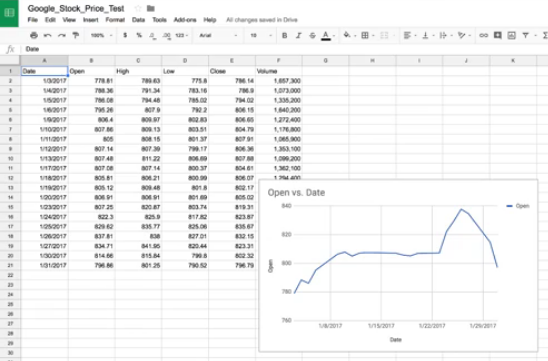
\includegraphics[width=0.6\linewidth,keepaspectratio]{lstm47}
\end{center}
As shown in Test file, we need to predict the upward trend. We won't get the spike predicted but just the trend.
\end{frame}

%%%%%%%%%%%%%%%%%%%%%%%%%%%%%%%%%%%%%%%%%%%%%%%%%%
\begin{frame}[fragile] \frametitle{Prediction}

With following code we are going to predict Jan 2017 stock prices. Each day in Jan, will need 60 previous prices ready. So we will need both Training ad Testing set to prepare this data, to be used for prediction. One idea could be to concatenate training\_set and the testing set. But the problem is that the training set is scaled by particuler Scaler obj, but the testing set is not. Mismatch. Need to work with original dataset merged, then starting with Jan, and its backward 60 timesteps. We are not changing actual test values.
\begin{lstlisting}
dataset_total = pd.concat((dataset_train['Open'],dataset_test['Open']),axis = 0)
inputs = dataset_total[len(dataset_total) - len(dataset_test) - 60: ].values # Jan first day, Jan 3rd, 60 days before, till end
\end{lstlisting}
Reshape with -1,1 is used to get values in single column. So, previous (80,) shape changed to (80,1).
\end{frame}



%%%%%%%%%%%%%%%%%%%%%%%%%%%%%%%%%%%%%%%%%%%%%%%%%%
\begin{frame}[fragile] \frametitle{Prediction}
\begin{itemize}
\item Scaling normalization with original sc obj. 
\item Dont recreate as same ratio is needed in prediction.
\item Prep x test. y test is not needed.
\item Only 20 precitions to be made, so range ends at $60+20=80$. 
\item Make it 3d as before. 
\item Need to inverse scaling on predcition to get the actual stock prices.
\end{itemize}
\begin{lstlisting}
inputs = sc.transform(inputs)
x_test = []

for i in range(60,80):
    x_test.append(inputs[i-60: i,0])
x_test = np.array(x_test)
x_test = np.reshape(x_test,(x_test.shape[0],x_test.shape[1],1))
predicted_stock_price = regressor.predict(x_test)
predicted_stock_price = sc.inverse_transform(predicted_stock_price)
\end{lstlisting}

\end{frame}


%%%%%%%%%%%%%%%%%%%%%%%%%%%%%%%%%%%%%%%%%%%%%%%%%%
\begin{frame}[fragile] \frametitle{Visualize}
\begin{lstlisting}
plt.plot(real_stock_price,color = 'red',label="Real Google Stock Price")
plt.plot(predicted_stock_price,color = 'blue',label="Predicted Google Stock Price")
plt.title("Google Stock Price Prediction")
plt.xlabel("Time")
plt.ylabel("Stock Price")
plt.legend()
plt.show()
\end{lstlisting}
\begin{center}
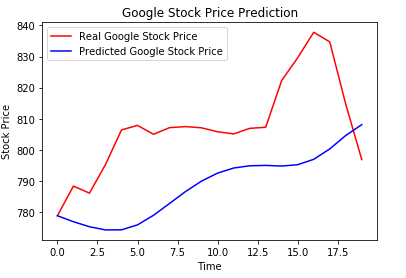
\includegraphics[width=0.5\linewidth,keepaspectratio]{lstm48}
\end{center}
\end{frame}


%%%%%%%%%%%%%%%%%%%%%%%%%%%%%%%%%%%%%%%%%%%%%%%%%%
\begin{frame}[fragile] \frametitle{Comments}
\begin{center}
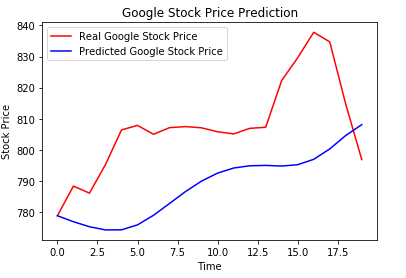
\includegraphics[width=0.5\linewidth,keepaspectratio]{lstm48}
\end{center}
\begin{itemize}
\item Model lags behind as it does not capture (spike) non linear change well.
\item It acts like smooth average curve (60 days moving average)
\item Trend looks fine. Even the last downward one.
\end{itemize}
\end{frame}









%%%%%%%%%%%%%%%%%%%%%%%%%%%%%%%%%%%%%%%%%%%%%%%%%%%
\begin{frame}[fragile] \frametitle{Household Power Consumption Prediction}
\begin{itemize}
\item Dataset:  https://archive.ics.uci.edu/ml/datasets/Individual+household

+electric+power+consumption\#
\item The task here will be to be able to predict values for a timeseries : the history of 2 million minutes of a household's power consumption. 
\item We are going to use a multi-layered LSTM recurrent neural network to predict the last value of a sequence of values. 
\item Put another way, given 49 timesteps of consumption, what will be the 50th value?
\end{itemize}
(Ref: Victor Schmidt https://github.com/Vict0rSch)
\end{frame}


%%%%%%%%%%%%%%%%%%%%%%%%%%%%%%%%%%%%%%%%%%%%%%%%%%
\begin{frame}[fragile] \frametitle{Imports}

\begin{lstlisting}
import matplotlib.pyplot as plt
import numpy as np
import time
import csv
from tf.keras.models import Sequential
from tf.keras.layers.core import Dense, Activation, Dropout
from tf.keras.layers.recurrent import LSTM
np.random.seed(1234)
\end{lstlisting}
Last thing is that for reproductibility, a seed is used in numpy's random.
\end{frame}

%%%%%%%%%%%%%%%%%%%%%%%%%%%%%%%%%%%%%%%%%%%%%%%%%%
\begin{frame}[fragile] \frametitle{Loading Data}

\begin{itemize}
\item The initial file contains lots of different pieces of data. 
\item We will here focus on a single value : a house's Global\_active\_power history, minute by minute for almost 4 years. 
\item This means roughly 2 million points. 
\item Some values are missing, this is why we try to load the values as floats into the list and if the value is not a number ( missing values are marked with a ?)  we simply ignore them.
\item If we do not want to load the entire dataset, there is a condition to stop loading the data when a certain ratio is reached. For now its FULL, ie 1.0
\end{itemize}
\end{frame}

%%%%%%%%%%%%%%%%%%%%%%%%%%%%%%%%%%%%%%%%%%%%%%%%%%
\begin{frame}[fragile] \frametitle{Loading Data}

\begin{lstlisting}
def data_power_consumption(path_to_dataset='household_power_consumption.txt', sequence_length=50, ratio=1.0):
    max_values = ratio * 2049280
    with open(path_to_dataset) as f:
        data = csv.reader(f, delimiter=";")
        power = []
        nb_of_values = 0
        for line in data:
            try:
                power.append(float(line[2]))
                nb_of_values += 1
            except ValueError:
                pass
            # 2049280.0 is the total number of valid values, i.e. ratio = 1.0
            if nb_of_values / 2049280.0 >= ratio:
                break
\end{lstlisting}

\end{frame}

%%%%%%%%%%%%%%%%%%%%%%%%%%%%%%%%%%%%%%%%%%%%%%%%%%
\begin{frame}[fragile] \frametitle{Loading Data}
\begin{itemize}
\item Once all the datapoints are loaded as one large timeseries, we have to split it into examples. 
\item Again, one example is made of a sequence of 50 values. Using the first 49, we are going to try and predict the 50th.
\item Moreover, we'll do this for every minute given the 49 previous ones so we use a sliding buffer of size 50.
\end{itemize}

\end{frame}

%%%%%%%%%%%%%%%%%%%%%%%%%%%%%%%%%%%%%%%%%%%%%%%%%%
\begin{frame}[fragile] \frametitle{Loading Data}

\begin{lstlisting}
def data_power_consumption(path_to_dataset='household_power_consumption.txt', sequence_length=50, ratio=1.0):
	:
	:
    result = []
    for index in range(len(power) - sequence_length):
        result.append(power[index: index + sequence_length])
    result = np.array(result) # shape (2049230, 50)	
    
    result_mean = result.mean()
    result -= result_mean
    print "Shift : ", result_mean
    print "Data  : ", result.shape    
\end{lstlisting}
Simply center the data to have a 0 mean.
\end{frame}

%%%%%%%%%%%%%%%%%%%%%%%%%%%%%%%%%%%%%%%%%%%%%%%%%%
\begin{frame}[fragile] \frametitle{Split Train Test Data}
\begin{itemize}
\item Here we select 10\% of the data as test and 90\% to train. 
\item We also select the last value of each example to be the target, the rest being the sequence of inputs.
\end{itemize}
\end{frame}

%%%%%%%%%%%%%%%%%%%%%%%%%%%%%%%%%%%%%%%%%%%%%%%%%%
\begin{frame}[fragile] \frametitle{Split Train Test Data}

\begin{lstlisting}
def data_power_consumption(path_to_dataset='household_power_consumption.txt', sequence_length=50, ratio=1.0):
	:
	:
    row = int(round(0.9 * result.shape[0]))
    train = result[:row, :]
    np.random.shuffle(train)
    X_train = train[:, :-1]
    y_train = train[:, -1]
    X_test = result[row:, :-1]
    y_test = result[row:, -1]
\end{lstlisting}
\end{frame}


%%%%%%%%%%%%%%%%%%%%%%%%%%%%%%%%%%%%%%%%%%%%%%%%%%
\begin{frame}[fragile] \frametitle{Split Train Test Data}
\begin{itemize}
\item We shuffle the training examples so that we train in no particular order and the distribution is uniform (for the batch calculation of the loss) 
\item but not the test set so that we can visualize our predictions with real signals.
\item we reshape the inputs to have dimensions (\#examples, \#values in sequences, dim. of each value). 
\item Here each value is 1-dimensional, they are only one measure (of power consumption at time t). 
\item However if we were to predict speed vectors they could be 3 dimensional for instance.
\end{itemize}
\end{frame}

%%%%%%%%%%%%%%%%%%%%%%%%%%%%%%%%%%%%%%%%%%%%%%%%%%
\begin{frame}[fragile] \frametitle{Split Train Test Data}

\begin{lstlisting}
def data_power_consumption(path_to_dataset='household_power_consumption.txt', sequence_length=50, ratio=1.0):
	:
	:
    X_train = np.reshape(X_train, (X_train.shape[0], X_train.shape[1], 1))
    X_test = np.reshape(X_test, (X_test.shape[0], X_test.shape[1], 1))
    
    return [X_train, y_train, X_test, y_test]
\end{lstlisting}
\end{frame}


%%%%%%%%%%%%%%%%%%%%%%%%%%%%%%%%%%%%%%%%%%%%%%%%%%
\begin{frame}[fragile] \frametitle{Building the model}
\begin{itemize}
\item So here we are going to build our Sequential model. 
\item This means we're going to stack layers in this object.
\item Also, layers is the list containing the sizes of each layer.
\item We are therefore going to have a network with 1-dimensional input, two hidden layers of sizes 50 and 100 and eventually a 1-dimensional output layer.
\end{itemize}
\end{frame}

%%%%%%%%%%%%%%%%%%%%%%%%%%%%%%%%%%%%%%%%%%%%%%%%%%
\begin{frame}[fragile] \frametitle{Building the model}
\begin{lstlisting}
def build_model():

    model = Sequential()
    layers = [1, 50, 100, 1]
\end{lstlisting}
\end{frame}


%%%%%%%%%%%%%%%%%%%%%%%%%%%%%%%%%%%%%%%%%%%%%%%%%%
\begin{frame}[fragile] \frametitle{Building the model}
\begin{itemize}
\item After the model is initialized, we create a first layer, in this case an LSTM layer. 
\item Here we use the default parameters so it behaves as a standard recurrent layer. 
\item Since our input is of 1 dimension, we declare that it should expect an input\_dim of 1. 
\item Then we say we want layers[1] units in this layer. We also add 20\% Dropout in this layer.
\end{itemize}
\end{frame}

%%%%%%%%%%%%%%%%%%%%%%%%%%%%%%%%%%%%%%%%%%%%%%%%%%
\begin{frame}[fragile] \frametitle{Building the model}
\begin{lstlisting}
    model.add(LSTM(
            layers[1],
            input_shape=(None, 1),
            return_sequences=True))
    model.add(Dropout(0.2))
\end{lstlisting}    
\end{frame}

%%%%%%%%%%%%%%%%%%%%%%%%%%%%%%%%%%%%%%%%%%%%%%%%%%
\begin{frame}[fragile] \frametitle{Building the model}
Second layer is even simpler to create, we just say how many units we want (layers[2]) and Keras takes care of the rest.
\begin{lstlisting}
    model.add(LSTM(
            layers[2],
            return_sequences=False))
    model.add(Dropout(0.2))
\end{lstlisting}    
\end{frame}

%%%%%%%%%%%%%%%%%%%%%%%%%%%%%%%%%%%%%%%%%%%%%%%%%%
\begin{frame}[fragile] \frametitle{Building the model}
The last layer we use is a Dense layer ( = feedforward). Since we are doing a regression, its activation is linear.
\begin{lstlisting}
    model.add(Dense(
            layers[3]))
    model.add(Activation("linear"))
\end{lstlisting}    
\end{frame}

%%%%%%%%%%%%%%%%%%%%%%%%%%%%%%%%%%%%%%%%%%%%%%%%%%
\begin{frame}[fragile] \frametitle{Compile the model}
Lastly, we compile the model using a Mean Square Error (again, it's standard for regression) and the RMSprop optimizer.
\begin{lstlisting}
    start = time.time()
    model.compile(loss="mse", optimizer="rmsprop")
    print "Compilation Time : ", time.time() - start
    return model
\end{lstlisting}    
\end{frame}

%%%%%%%%%%%%%%%%%%%%%%%%%%%%%%%%%%%%%%%%%%%%%%%%%%
\begin{frame}[fragile] \frametitle{Return Sequence}
\begin{center}
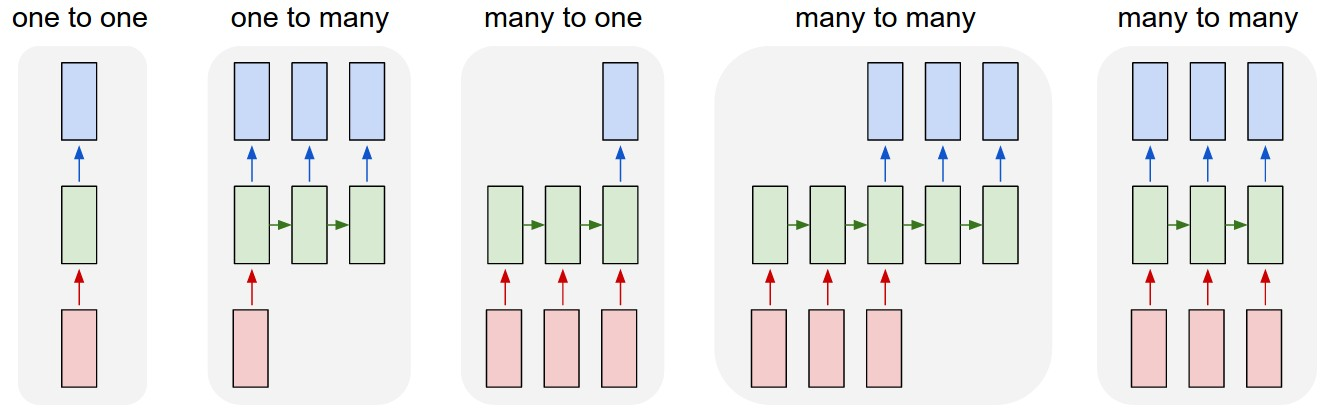
\includegraphics[width=0.7\linewidth,keepaspectratio]{rnnkr1}
\end{center}
\begin{itemize}
\item The difference between $return\_sequence=True$ and $return\_sequence=False$ is that 
\item In the first case the network behaves as in the 5th illustration (second many to many) and
\item In the latter it behaves as the 3rd, many to one.
\end{itemize}
\end{frame}

%%%%%%%%%%%%%%%%%%%%%%%%%%%%%%%%%%%%%%%%%%%%%%%%%%
\begin{frame}[fragile] \frametitle{Return Sequence}
\begin{center}
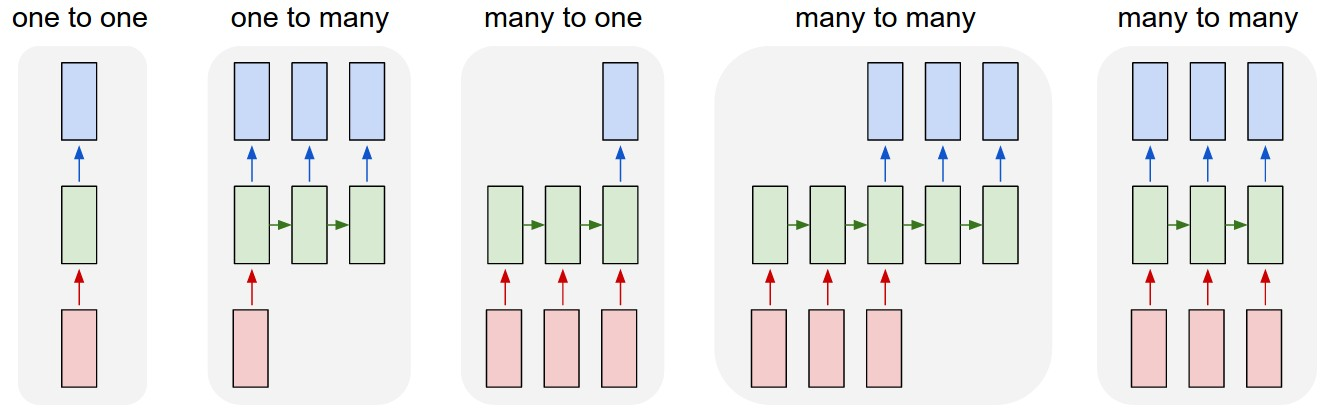
\includegraphics[width=0.7\linewidth,keepaspectratio]{rnnkr1}
\end{center}
\begin{itemize}
\item In our case, the first LSTM layer returns sequences because we want it to transfer its information both to the next layer (upwards in the chart) and 
\item to itself for the next timestep (arrow to the right).
\end{itemize}
\end{frame}

%%%%%%%%%%%%%%%%%%%%%%%%%%%%%%%%%%%%%%%%%%%%%%%%%%
\begin{frame}[fragile] \frametitle{Return Sequence}
\begin{center}
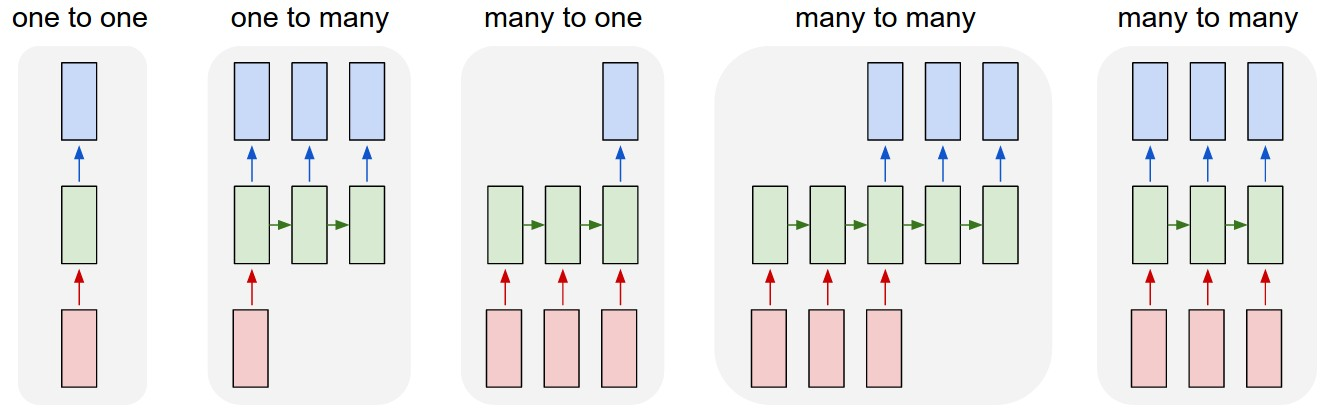
\includegraphics[width=0.7\linewidth,keepaspectratio]{rnnkr1}
\end{center}
\begin{itemize}
\item However for the second one, we just expect its last sequence prediction to be compared to the target. 
\item This means for inputs (0 to sequence\_length - 2) the prediction is only passed to the layer itself for the next timestep and not as an input to the next ( = output) layer.
\item However the (sequence\_length - 1)th input is passed forward to the Dense layer for the loss computation against the target.
\end{itemize}
\end{frame}

%%%%%%%%%%%%%%%%%%%%%%%%%%%%%%%%%%%%%%%%%%%%%%%%%%
\begin{frame}[fragile] \frametitle{Return Sequence}
More explanation, with an example, where sequence\_length=3.
\begin{itemize}
\item In this case the aim would be to predict the 4th value and compute the loss against the real 4th value, the target.
\item The first example value is fed to the network from the input
\begin{itemize}
\item The first hidden layer's activation is computed and passed both to the second hidden layer and to itself
\item The second hidden layer takes as input the first hidden layer's activation, computes its own activation and passes it only to itself
\end{itemize}
\end{itemize}
\end{frame}

%%%%%%%%%%%%%%%%%%%%%%%%%%%%%%%%%%%%%%%%%%%%%%%%%%
\begin{frame}[fragile] \frametitle{Return Sequence}
\begin{itemize}
\item The second example of the same sequence is fed from the input
\begin{itemize}
\item The first hidden layer takes as input both this value and its own previous prediction from the first timestep. The computed activation is fed again both to the second layer and to the first hidden layer itself
\item The second layer behaves likewise: it takes its previous prediction and the first hidden layer's output as inputs and outputs an activation. This activation, once again, is fed to the second hidden layer for the next timestep
\end{itemize}
\end{itemize}
\end{frame}

%%%%%%%%%%%%%%%%%%%%%%%%%%%%%%%%%%%%%%%%%%%%%%%%%%
\begin{frame}[fragile] \frametitle{Return Sequence}
\begin{itemize}
\item The last value of the sequence is input into the network
\begin{itemize}
\item The first hidden layer behaves as before (2.a)
\item The second layer also behaves as before (2.b) except that this time, its activation is also passed to the last, Dense layer.
\item The Dense layer computes its activation from the second hidden layer's activation. This activation is the prediction our network does for the 4th timestep.
\end{itemize}
\end{itemize}
\end{frame}

%%%%%%%%%%%%%%%%%%%%%%%%%%%%%%%%%%%%%%%%%%%%%%%%%%
\begin{frame}[fragile] \frametitle{Return Sequence}
To conclude
\begin{itemize}
\item The fact that return\_sequence=True for the first layer means that its output is always fed to the second layer. As a whole regarding time, all its activations can be seen as the sequence of prediction this first layer has made from the input sequence.
\item On the other hand, return\_sequence=False for the second layer because its output is only fed to the next layer at the end of the sequence. As a whole regarding time, it does not output a prediction for the sequence but one only prediction-vector (of size layer[2]) for the whole input sequence. 
\item The linear Dense layer is used to aggregate all the information from this prediction-vector into one single value, the predicted 4th timestep of the sequence.
\end{itemize}
\end{frame}

%%%%%%%%%%%%%%%%%%%%%%%%%%%%%%%%%%%%%%%%%%%%%%%%%%
\begin{frame}[fragile] \frametitle{To go further}
\begin{itemize}
\item Had we stacked three recurrent hidden layers, we'd have set return\_sequence=True to the second hidden layer and return\_sequence=False to the last. 
\item In other words, return\_sequence=False is used as an interface from recurrent to feedforward layers (dense or convolutionnal).

\item Also, if the output had a $dimension > 1$, we'd only change the size of the Dense layer.
\end{itemize}
\end{frame}

%%%%%%%%%%%%%%%%%%%%%%%%%%%%%%%%%%%%%%%%%%%%%%%%%%
\begin{frame}[fragile] \frametitle{Running the model}
\begin{lstlisting}
def run_network(model=None, data=None):
    epochs = 1
    ratio = 0.5
    path_to_dataset = 'household_power_consumption.txt'
    
    if data is None:
        print 'Loading data... '
        X_train, y_train, X_test, y_test = data_power_consumption(
                path_to_dataset, sequence_length, ratio)
    else:
        X_train, y_train, X_test, y_test = data
    
    print '\nData Loaded. Compiling...\n'
    
    if model is None:
        model = build_model()
\end{lstlisting}   
To be as modular as possible we start with checking whether or not data and model values were provided. 
\end{frame}


%%%%%%%%%%%%%%%%%%%%%%%%%%%%%%%%%%%%%%%%%%%%%%%%%%
\begin{frame}[fragile] \frametitle{Running the model}
\begin{lstlisting}
def run_network(model=None, data=None):
	:
	:
	try:
        model.fit(
            X_train, y_train,
            batch_size=512, nb_epoch=epochs, validation_split=0.05)
        predicted = model.predict(X_test)
        predicted = np.reshape(predicted, (predicted.size,))
    except KeyboardInterrupt:
        print 'Training duration (s) : ', time.time() - global_start_time
        return model, y_test, 0
\end{lstlisting}           
\end{frame}

%%%%%%%%%%%%%%%%%%%%%%%%%%%%%%%%%%%%%%%%%%%%%%%%%%
\begin{frame}[fragile] \frametitle{More about Predictions}
\begin{itemize}
\item By construction X\_test is an array with 49 columns (timesteps). The list [ X\_test[i][0] ] is the entire signal (minus the last 49 values) from which it was built since we've used a 1-timestep sliding buffer.
\item X\_test[0] is the first sequence, that is to say the first 49 values of the original signal.
\end{itemize}
\end{frame}


%%%%%%%%%%%%%%%%%%%%%%%%%%%%%%%%%%%%%%%%%%%%%%%%%%
\begin{frame}[fragile] \frametitle{More about Predictions}
\begin{itemize}
\item predict(X\_test[0]) is therefore the prediction for the 50th value and its associated target is y\_test[0]. 
\item Moreover, by construction, y\_test[0] = X\_test[1][48] = X\_test[2][47] = \ldots
\item Then predict(X\_test[1]) is the prediction of the 51th value, associated with y\_test[1] as a target.
\end{itemize}
\end{frame}

%%%%%%%%%%%%%%%%%%%%%%%%%%%%%%%%%%%%%%%%%%%%%%%%%%
\begin{frame}[fragile] \frametitle{More about Predictions}
\begin{itemize}
\item Therefore predict(X\_test) is the predicted signal, one step ahead, and y\_test is its target.
\item predict(X\_test) is a list of lists (in fact a 2-dimensional numpy array) with one value, therefore we reshape it so that it simply is a list of values (1-dimensional numpy array).
\end{itemize}
\end{frame}


%%%%%%%%%%%%%%%%%%%%%%%%%%%%%%%%%%%%%%%%%%%%%%%%%%
\begin{frame}[fragile] \frametitle{Running the model}
Lastly we plot the result of the prediction for the first 100 timesteps and return model, y\_test and the predicted values.
\begin{lstlisting}
def run_network(model=None, data=None):
	:
	:
    try:
        fig = plt.figure()
        ax = fig.add_subplot(111)
        ax.plot(y_test[:100, 0])
        plt.plot(predicted[:100, 0])
        plt.show()
    except Exception as e:
        print str(e)
    print 'Training duration (s) : ', time.time() - global_start_time
    return model, y_test, predicted
    
if __name__ == '__main__':
run_network()
\end{lstlisting}           
\end{frame}

%%%%%%%%%%%%%%%%%%%%%%%%%%%%%%%%%%%%%%%%%%%%%%%%%%%
\begin{frame}
  \begin{center}
    {\Large LSTM with Keras}
    
(Ref: Time Series Forecasting with the Long Short-Term Memory Network in Python - Jason Brownlee)
  \end{center}
\end{frame}



%%%%%%%%%%%%%%%%%%%%%%%%%%%%%%%%%%%%%%%%%%%%%%%%%%
\begin{frame}[fragile] \frametitle{Dataset}
\begin{itemize}
\item Shampoo Sales: https://datamarket.com/data/set/22r0/sales-of-shampoo-over-a-three-year-period
\item The monthly number of sales of shampoo over a 3-year period.
\item Note that you may need to delete the footer information added by DataMarket.
\end{itemize}
\begin{lstlisting}
# load and plot dataset
from pandas import read_csv
from pandas import datetime
from matplotlib import pyplot
# load dataset
def parser(x):
	return datetime.strptime('190'+x, '%Y-%m')
series = read_csv('shampoo-sales.csv', header=0, parse_dates=[0], index_col=0, squeeze=True, date_parser=parser)
\end{lstlisting}   
\end{frame}

%%%%%%%%%%%%%%%%%%%%%%%%%%%%%%%%%%%%%%%%%%%%%%%%%%
\begin{frame}[fragile] \frametitle{Dataset}
Print first few rows
\begin{lstlisting}
# summarize first few rows
print(series.head())

#Month
1901-01-01 266.0
1901-02-01 145.9
1901-03-01 183.1
1901-04-01 119.3
1901-05-01 180.3
Name: Sales, dtype: float64
\end{lstlisting}   
\end{frame}

%%%%%%%%%%%%%%%%%%%%%%%%%%%%%%%%%%%%%%%%%%%%%%%%%%
\begin{frame}[fragile] \frametitle{Dataset}
Plot 
\begin{lstlisting}
series.plot()
pyplot.show()
\end{lstlisting}   
\begin{center}
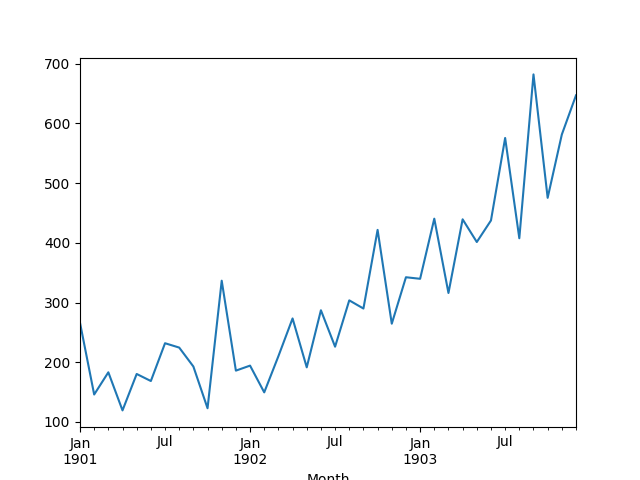
\includegraphics[width=0.5\linewidth,keepaspectratio]{rnnkr2}
\end{center}
A line plot of the series is then created showing a clear increasing trend.
\end{frame}

%%%%%%%%%%%%%%%%%%%%%%%%%%%%%%%%%%%%%%%%%%%%%%%%%%%
%\begin{frame}[fragile] \frametitle{Dataset}
%\begin{itemize}
%\item We will split the Shampoo Sales dataset into two parts: a training and a test set.
%\item The first two years of data will be taken for the training dataset and the remaining one year of data will be used for the test set.
%\item Models will be developed using the training dataset and will make predictions on the test dataset.
%\end{itemize}
%\begin{lstlisting}
%# split data into train and test
%X = series.values
%train, test = X[0:-12], X[-12:]
%\end{lstlisting}   
%\end{frame}
%%
%%%%%%%%%%%%%%%%%%%%%%%%%%%%%%%%%%%%%%%%%%%%%%%%%%%%
%%\begin{frame}[fragile] \frametitle{Model}
%%\begin{itemize}
%%\item A rolling forecast scenario will be used, also called walk-forward model validation.
%%\item For evaluation: Each time step of the test dataset will be walked one at a time. 
%%\item A model will be used to make a forecast for the time step, then the actual expected value from the test set will be taken and made available to the model for the forecast on the next time step.
%%\item This mimics a real-world scenario where new Shampoo Sales observations would be available each month and used in the forecasting of the following month.
%%\end{itemize}
%%\begin{lstlisting}
%%# split data into train and test
%%X = series.values
%%train, test = X[0:-12], X[-12:]
%%\end{lstlisting}   
%%\end{frame}
%%
%%%%%%%%%%%%%%%%%%%%%%%%%%%%%%%%%%%%%%%%%%%%%%%%%%%%
%%\begin{frame}[fragile] \frametitle{Model}
%%\begin{itemize}
%%\item Finally, all forecasts on the test dataset will be collected and an error score calculated to summarize the skill of the model. 
%%\item The root mean squared error (RMSE) will be used as it punishes large errors and results in a score that is in the same units as the forecast data, namely monthly shampoo sales.
%%\end{itemize}
%%\begin{lstlisting}
%%from sklearn.metrics import mean_squared_error
%%rmse = sqrt(mean_squared_error(test, predictions))
%%print('RMSE: %.3f' % rmse)
%%\end{lstlisting}   
%%\end{frame}
%%
%%%%%%%%%%%%%%%%%%%%%%%%%%%%%%%%%%%%%%%%%%%%%%%%%%%%
%%\begin{frame}[fragile] \frametitle{Persistence Model Forecast}
%%\begin{itemize}
%%\item A good baseline forecast for a time series with a linear increasing trend is a persistence forecast.
%%\item The persistence forecast is where the observation from the prior time step (t-1) is used to predict the observation at the current time step (t).
%%\item We can implement this by taking the last observation from the training data and history accumulated by walk-forward validation and using that to predict the current time step.
%%\end{itemize}
%%\begin{lstlisting}
%%# make prediction
%%yhat = history[-1]
%%\end{lstlisting}   
%%We will accumulate all predictions in an array so that they can be directly compared to the test dataset.
%%\end{frame}
%%

%%%%%%%%%%%%%%%%%%%%%%%%%%%%%%%%%%%%%%%%%%%%%%%%%%
\begin{frame}[fragile] \frametitle{LSTM Data Preparation}
Before we can fit an LSTM model to the dataset, we must transform the data.
\begin{itemize}
\item Transform the time series into a supervised learning problem
\item Transform the time series data so that it is stationary.
\item Transform the observations to have a specific scale.
\end{itemize}
\end{frame}

%%%%%%%%%%%%%%%%%%%%%%%%%%%%%%%%%%%%%%%%%%%%%%%%%%
\begin{frame}[fragile] \frametitle{Transform the time series into a supervised learning problem}
\begin{itemize}
\item The LSTM model in Keras assumes that your data is divided into input (X) and output (y) components.
\item For a time series problem, we can achieve this by using the observation from the last time step (t-1) as the input and the observation at the current time step (t) as the output.
\item We can achieve this using the shift() function in Pandas that will push all values in a series down by a specified number places. 
\item We require a shift of 1 place, which will become the input variables. 
\item The time series as it stands will be the output variables.
\item Basically, two seqeunces, one input and one output
\end{itemize}
\end{frame}

%%%%%%%%%%%%%%%%%%%%%%%%%%%%%%%%%%%%%%%%%%%%%%%%%%
\begin{frame}[fragile] \frametitle{Transform the time series into a supervised learning problem}
\begin{itemize}
\item We can then concatenate these two series together to create a DataFrame ready for supervised learning. 
\item Due to shift the input serie's first element will come below output series' 2nd element.
\item So Outputs 2nd elements input will be Inputs 2nd element (which was actually the first element), thus Outputs $t$ has inputs $t-1$
\item So, the first position in the input series will be blank, or NaN. 
\item We will replace these NaN values with 0 values, which the LSTM model will have to learn as ``the start of the series'' or `'I have no data here,'' as a month with zero sales on this dataset has not been observed.
\end{itemize}
\end{frame}

%%%%%%%%%%%%%%%%%%%%%%%%%%%%%%%%%%%%%%%%%%%%%%%%%%
\begin{frame}[fragile] \frametitle{Transform the time series into a supervised learning problem}
\begin{itemize}
\item The code below defines a helper function to do this called timeseries\_to\_supervised(). 
\item It takes a NumPy array of the raw time series data and a lag or number of shifted series to create and use as inputs.
\end{itemize}
\begin{lstlisting}
# frame a sequence as a supervised learning problem
def timeseries_to_supervised(data, lag=1):
	df = DataFrame(data)
	columns = [df.shift(i) for i in range(1, lag+1)]
	columns.append(df)
	df = concat(columns, axis=1)
	df.fillna(0, inplace=True)
	return df
\end{lstlisting}   
We can test this function with our loaded Shampoo Sales dataset and convert it into a supervised learning problem.
\end{frame}

%%%%%%%%%%%%%%%%%%%%%%%%%%%%%%%%%%%%%%%%%%%%%%%%%%
\begin{frame}[fragile] \frametitle{Transform the time series into a supervised learning problem}
We can test this function with our loaded Shampoo Sales dataset and convert it into a supervised learning problem.
\begin{lstlisting}
# transform to supervised learning
X = series.values
supervised = timeseries_to_supervised(X, 1)
print(supervised.head())

            0           0
0    0.000000  266.000000
1  266.000000  145.899994
2  145.899994  183.100006
3  183.100006  119.300003
4  119.300003  180.300003
\end{lstlisting}   
\end{frame}

%%%%%%%%%%%%%%%%%%%%%%%%%%%%%%%%%%%%%%%%%%%%%%%%%%
\begin{frame}[fragile] \frametitle{Transform Time Series to Stationary}
\begin{itemize}
\item The Shampoo Sales dataset is not stationary.
\item It  is dependent on the time. Specifically, there is an increasing trend in the data.
\item Stationary data is easier to model and will very likely result in more skillful forecasts.
\item The trend can be removed from the observations, then added back to forecasts later to return the prediction to the original scale and calculate a comparable error score.
\item A standard way to remove a trend is by differencing the data. 
\end{itemize}

\end{frame}

%%%%%%%%%%%%%%%%%%%%%%%%%%%%%%%%%%%%%%%%%%%%%%%%%%
\begin{frame}[fragile] \frametitle{Transform Time Series to Stationary}
\begin{itemize}
\item That is the observation from the previous time step (t-1) is subtracted from the current observation (t). 
\item This removes the trend and we are left with a difference series, or the changes to the observations from one time step to the next.
\item We can achieve this automatically using the diff() function in pandas.
\item Alternatively, we can get finer grained control and write our own function to do this, which is preferred for its flexibility in this case.
\end{itemize}

\end{frame}

%%%%%%%%%%%%%%%%%%%%%%%%%%%%%%%%%%%%%%%%%%%%%%%%%%
\begin{frame}[fragile] \frametitle{Transform Time Series to Stationary}
\begin{itemize}
\item Below is a function called difference() that calculates a differenced series. 
\item Note that the first observation in the series is skipped as there is no prior observation with which to calculate a differenced value.
\end{itemize}
\begin{lstlisting}
# create a differenced series
def difference(dataset, interval=1):
	diff = list()
	for i in range(interval, len(dataset)):
		value = dataset[i] - dataset[i - interval]
		diff.append(value)
	return Series(diff)
\end{lstlisting}   
\end{frame}

%%%%%%%%%%%%%%%%%%%%%%%%%%%%%%%%%%%%%%%%%%%%%%%%%%
\begin{frame}[fragile] \frametitle{Transform Time Series to Stationary}
We also need to invert this process in order to take forecasts made on the differenced series back into their original scale.
\begin{lstlisting}
# invert differenced value
def inverse_difference(history, yhat, interval=1):
	return yhat + history[-interval]
\end{lstlisting}   

\end{frame}

%%%%%%%%%%%%%%%%%%%%%%%%%%%%%%%%%%%%%%%%%%%%%%%%%%
\begin{frame}[fragile] \frametitle{Transform Time Series to Stationary}
We can test out these functions by differencing the whole series, then returning it to the original scale, as follows:
\begin{lstlisting}
# transform to be stationary
differenced = difference(series, 1)
print(differenced.head())
# invert transform
inverted = list()
for i in range(len(differenced)):
	value = inverse_difference(series, differenced[i], len(series)-i)
	inverted.append(value)
inverted = Series(inverted)
print(inverted.head())
\end{lstlisting}   
Note that the first observation in the original dataset was removed from the inverted difference data. 
\end{frame}

%%%%%%%%%%%%%%%%%%%%%%%%%%%%%%%%%%%%%%%%%%%%%%%%%%
\begin{frame}[fragile] \frametitle{Transform Time Series to Scale}
\begin{itemize}
\item Like other neural networks, LSTMs expect data to be within the scale of the activation function used by the network.
\item The default activation function for LSTMs is the hyperbolic tangent (tanh), which outputs values between -1 and 1. 
\item This is the preferred range for the time series data.
\item We can transform the dataset to the range [-1, 1] using the MinMaxScaler class. 
\end{itemize}
\end{frame}

%%%%%%%%%%%%%%%%%%%%%%%%%%%%%%%%%%%%%%%%%%%%%%%%%%
\begin{frame}[fragile] \frametitle{Transform Time Series to Scale}
\begin{itemize}
\item Like other scikit-learn transform classes, it requires data provided in a matrix format with rows and columns. 
\item Therefore, we must reshape our NumPy arrays before transforming.
\end{itemize}
\begin{lstlisting}
# transform scale
X = series.values
X = X.reshape(len(X), 1)
scaler = MinMaxScaler(feature_range=(-1, 1))
scaler = scaler.fit(X)
scaled_X = scaler.transform(X)
\end{lstlisting}   
\end{frame}

%%%%%%%%%%%%%%%%%%%%%%%%%%%%%%%%%%%%%%%%%%%%%%%%%%
\begin{frame}[fragile] \frametitle{Transform Time Series to Scale}
Again, we must invert the scale on forecasts to return the values back to the original scale so that the results can be interpreted and a comparable error score can be calculated.
\begin{lstlisting}
# invert transform
inverted_X = scaler.inverse_transform(scaled_X)
\end{lstlisting}   
\end{frame}

%%%%%%%%%%%%%%%%%%%%%%%%%%%%%%%%%%%%%%%%%%%%%%%%%%
\begin{frame}[fragile] \frametitle{Transform Time Series to Scale}
Putting all of this together, the example below transforms the scale of the Shampoo Sales data.
\begin{lstlisting}
# transform scale
X = series.values
X = X.reshape(len(X), 1)
scaler = MinMaxScaler(feature_range=(-1, 1))
scaler = scaler.fit(X)
scaled_X = scaler.transform(X)
scaled_series = Series(scaled_X[:, 0])
print(scaled_series.head())
# invert transform
inverted_X = scaler.inverse_transform(scaled_X)
inverted_series = Series(inverted_X[:, 0])
print(inverted_series.head())
\end{lstlisting}   
\end{frame}

%%%%%%%%%%%%%%%%%%%%%%%%%%%%%%%%%%%%%%%%%%%%%%%%%%
\begin{frame}[fragile] \frametitle{LSTM Model Development}
\begin{itemize}
\item By default, an LSTM layer in Keras maintains state between data within one batch. 
\item A batch of data is a fixed-sized number of rows from the training dataset that defines how many patterns to process before updating the weights of the network. 
\item State in the LSTM layer between batches is cleared by default, therefore we must make the LSTM stateful. 
\item This gives us fine-grained control over when state of the LSTM layer is cleared, by calling the reset\_states() function.
\end{itemize}
\end{frame}

%%%%%%%%%%%%%%%%%%%%%%%%%%%%%%%%%%%%%%%%%%%%%%%%%%
\begin{frame}[fragile] \frametitle{LSTM Model Development}
The LSTM layer expects input to be in a matrix with the dimensions: [samples, time steps, features].
\begin{itemize}
\item 
    Samples: These are independent observations from the domain, typically rows of data.
\item Time steps: These are separate time steps of a given variable for a given observation.
\item  Features: These are separate measures observed at the time of observation.
\end{itemize}
\end{frame}

%%%%%%%%%%%%%%%%%%%%%%%%%%%%%%%%%%%%%%%%%%%%%%%%%%
\begin{frame}[fragile] \frametitle{LSTM Model Development}
\begin{itemize}
\item 
    We will keep it simple and frame the problem as each time step in the original sequence is one separate sample, with one timestep and one feature.
    \item Given that the training dataset is defined as X inputs and y outputs, it must be reshaped into the Samples/TimeSteps/Features format, for example:
\end{itemize}
\begin{lstlisting}
X, y = train[:, 0:-1], train[:, -1]
X = X.reshape(X.shape[0], 1, X.shape[1])
\end{lstlisting}   
\end{frame}

%%%%%%%%%%%%%%%%%%%%%%%%%%%%%%%%%%%%%%%%%%%%%%%%%%
\begin{frame}[fragile] \frametitle{LSTM Model Development}
\begin{itemize}
\item The shape of the input data must be specified in the LSTM layer using the ``batch\_input\_shape'' argument as a tuple that specifies the expected number of observations to read each batch, the number of time steps, and the number of features.
\item The batch size is often much smaller than the total number of samples. It, along with the number of epochs, defines how quickly the network learns the data (how often the weights are updated).
\item 
The final import parameter in defining the LSTM layer is the number of neurons, also called the number of memory units or blocks. This is a reasonably simple problem and a number between 1 and 5 should be sufficient.
\end{itemize}
\end{frame}

%%%%%%%%%%%%%%%%%%%%%%%%%%%%%%%%%%%%%%%%%%%%%%%%%%
\begin{frame}[fragile] \frametitle{LSTM Model Development}
\begin{itemize}
\item The line below creates a single LSTM hidden layer that also specifies the expectations of the input layer via the ``batch\_input\_shape'' argument.
\begin{lstlisting}
layer = LSTM(neurons, batch_input_shape=(batch_size, X.shape[1], X.shape[2]), stateful=True)
\end{lstlisting}   
\item The network requires a single neuron in the output layer with a linear activation to predict the number of shampoo sales at the next time step.
\end{itemize}
\end{frame}

%%%%%%%%%%%%%%%%%%%%%%%%%%%%%%%%%%%%%%%%%%%%%%%%%%
\begin{frame}[fragile] \frametitle{LSTM Model Development}
\begin{itemize}
\item In compiling the network, we must specify a loss function and optimization algorithm. We will use ``mean\_squared\_error'' as the loss function as it closely matches RMSE that we will are interested in, and the efficient ADAM optimization algorithm.
\item Using the Sequential Keras API to define the network, the below snippet creates and compiles the network.
\end{itemize}
\begin{lstlisting}
model = Sequential()
model.add(LSTM(neurons, batch_input_shape=(batch_size, X.shape[1], X.shape[2]), stateful=True))
model.add(Dense(1))
model.compile(loss='mean_squared_error', optimizer='adam')
\end{lstlisting} 
\end{frame}

%%%%%%%%%%%%%%%%%%%%%%%%%%%%%%%%%%%%%%%%%%%%%%%%%%
\begin{frame}[fragile] \frametitle{LSTM Model Development}
\begin{itemize}
\item Once compiled, it can be fit to the training data. Because the network is stateful, we must control when the internal state is reset. Therefore, we must manually manage the training process one epoch at a time across the desired number of epochs.

\item By default, the samples within an epoch are shuffled prior to being exposed to the network. Again, this is undesirable for the LSTM because we want the network to build up state as it learns across the sequence of observations. We can disable the shuffling of samples by setting ``shuffle'' to ``False``.

\item Also by default, the network reports a lot of debug information about the learning progress and skill of the model at the end of each epoch. We can disable this by setting the ``verbose'' argument to the level of ``0``.

\item We can then reset the internal state at the end of the training epoch, ready for the next training iteration.
\end{itemize}

\end{frame}

%%%%%%%%%%%%%%%%%%%%%%%%%%%%%%%%%%%%%%%%%%%%%%%%%%
\begin{frame}[fragile] \frametitle{LSTM Model Development}
Below is a loop that manually fits the network to the training data.
\begin{lstlisting}
for i in range(nb_epoch):
	model.fit(X, y, epochs=1, batch_size=batch_size, verbose=0, shuffle=False)
	model.reset_states()
\end{lstlisting} 

\end{frame}

%%%%%%%%%%%%%%%%%%%%%%%%%%%%%%%%%%%%%%%%%%%%%%%%%%
\begin{frame}[fragile] \frametitle{LSTM Model Development}
 fit\_lstm() that trains and returns an LSTM model.
\begin{lstlisting}
def fit_lstm(train, batch_size, nb_epoch, neurons):
	X, y = train[:, 0:-1], train[:, -1]
	X = X.reshape(X.shape[0], 1, X.shape[1])
	model = Sequential()
	model.add(LSTM(neurons, batch_input_shape=(batch_size, X.shape[1], X.shape[2]), stateful=True))
	model.add(Dense(1))
	model.compile(loss='mean_squared_error', optimizer='adam')
	for i in range(nb_epoch):
		model.fit(X, y, epochs=1, batch_size=batch_size, verbose=0, shuffle=False)
		model.reset_states()
	return model
\end{lstlisting} 
The batch\_size must be set to 1. This is because it must be a factor of the size of the training and test datasets.
\end{frame}

%%%%%%%%%%%%%%%%%%%%%%%%%%%%%%%%%%%%%%%%%%%%%%%%%%
\begin{frame}[fragile] \frametitle{LSTM Forecast}
\begin{itemize}
\item We can decide to fit the model once on all of the training data, then predict each new time step one at a time from the test data (we'll call this the fixed approach), or 
\item We can re-fit the model or update the model each time step of the test data as new observations from the test data are made available (we'll call this the dynamic approach).
\end{itemize}
\end{frame}

%%%%%%%%%%%%%%%%%%%%%%%%%%%%%%%%%%%%%%%%%%%%%%%%%%
\begin{frame}[fragile] \frametitle{LSTM Forecast}
\begin{itemize}
\item To make a forecast, we can call the predict() function on the model. This requires a 3D NumPy array input as an argument. In this case, it will be an array of one value, the observation at the previous time step.
\item The predict() function returns an array of predictions, one for each input row provided. Because we are providing a single input, the output will be a 2D NumPy array with one value.
\end{itemize}
\end{frame}

%%%%%%%%%%%%%%%%%%%%%%%%%%%%%%%%%%%%%%%%%%%%%%%%%%
\begin{frame}[fragile] \frametitle{LSTM Forecast}
\begin{itemize}
\item Given a fit model, a batch-size used when fitting the model (e.g. 1), and a row from the test data, the function will separate out the input data from the test row, reshape it, and return the prediction as a single floating point value.
\end{itemize}
\begin{lstlisting}
def forecast(model, batch_size, row):
	X = row[0:-1]
	X = X.reshape(1, 1, len(X))
	yhat = model.predict(X, batch_size=batch_size)
	return yhat[0,0]
\end{lstlisting} 
\end{frame}

%%%%%%%%%%%%%%%%%%%%%%%%%%%%%%%%%%%%%%%%%%%%%%%%%%
\begin{frame}[fragile] \frametitle{LSTM Forecast}
\begin{itemize}
\item During training, the internal state is reset after each epoch. While forecasting, we will not want to reset the internal state between forecasts. In fact, we would like the model to build up state as we forecast each time step in the test dataset.
\item 
This raises the question as to what would be a good initial state for the network prior to forecasting the test dataset.
\item 
In this tutorial, we will seed the state by making a prediction on all samples in the training dataset. In theory, the internal state should be set up ready to forecast the next time step.
\end{itemize}
\end{frame}


%%%%%%%%%%%%%%%%%%%%%%%%%%%%%%%%%%%%%%%%%%%%%%%%%%
\begin{frame}[fragile] \frametitle{LSTM Summary}
\begin{itemize}
\item Load the dataset from CSV file.
\item     Transform the dataset to make it suitable for the LSTM model, including:
\begin{itemize}
\item         Transforming the data to a supervised learning problem.
\item         Transforming the data to be stationary.
\item         Transforming the data so that it has the scale -1 to 1.
\end{itemize}
\item     Fitting a stateful LSTM network model to the training data.
\item     Evaluating the static LSTM model on the test data.
\item     Report the performance of the forecasts.

\end{itemize}
\end{frame}


%%%%%%%%%%%%%%%%%%%%%%%%%%%%%%%%%%%%%%%%%%%%%%%%%%
\begin{frame}[fragile] \frametitle{LSTM Summary}
Some things to note about the example:
\begin{itemize}
\item The scaling and inverse scaling behaviors have been moved to the functions scale() and invert\_scale() for brevity.
\item     The test data is scaled using the fit of the scaler on the training data, as is required to ensure the min/max values of the test data do not influence the model.
\item     The order of data transforms was adjusted for convenience to first make the data stationary, then a supervised learning problem, then scaled.
\item     Differencing was performed on the entire dataset prior to splitting into train and test sets for convenience. We could just as easily collect observations during the walk-forward validation and difference them as we go. I decided against it for readability.

\end{itemize}
\end{frame}

%
%
%%%%%%%%%%%%%%%%%%%%%%%%%%%%%%%%%%%%%%%%%%%%%%%%%%%%
%\begin{frame}[fragile] \frametitle{}
%
%
\includegraphics[width=\linewidth]{keras.pdf}
%
%\end{frame}
%
%%%%%%%%%%%%%%%%%%%%%%%%%%%%%%%%%%%%%%%%%%%%%%%%%%%%
%\begin{frame}[fragile] \frametitle{}
%\begin{itemize}
%\item For an input vector $x$ and a response $y$, we can view the network
%as simply being something like:
%\begin{align}
%z^1 &= W^1 a^0 + b^1 \\
%a^1 &= \sigma(z^1) \\
%z^2 &= W^2 a^1 + b^2 \\
%a^2 &= \sigma(z^2) \\
%z^3 &= W^3 a^2 + b^3 \\
%a^3 &= \sigma(z^3) \\
%\text{Cost} &= (y - a^3)^2
%\end{align}
%\item Each level can be described by a \textit{module}. 
%\item The $z$ layers
%are called linear layers, the $a$'s as sigmoid layers, and the last
%line is simply the cost function.
%\item The activation functions
%are now their own layers, which actually simplifies things mathematically.
%\end{itemize}
%\end{frame}
%
%%%%%%%%%%%%%%%%%%%%%%%%%%%%%%%%%%%%%%%%%%%%%%%%%%%%
%\begin{frame}[fragile] \frametitle{}
%
%Each type of module needs to be able to:
%\begin{itemize}
%\item take an input and return an output for the current tuning parameters
%\item calculate the matrix $\frac{\partial \text{output}_i}{\partial \text{input}_j}$
%\item calculate the set $\frac{\partial \text{output}_i}{\partial \text{parameters}_j}$
%\item store the tuning parameters
%\item update parameters from a minibatch
%\end{itemize}
%If all of these is readily implemented, one can simply chain together
%modules and have a built-in algorithm for learning from input data.
%
%\end{frame}
%
%%%%%%%%%%%%%%%%%%%%%%%%%%%%%%%%%%%%%%%%%%%%%%%%%%%%
%\begin{frame}[fragile] \frametitle{}
%
%An example, using the \textbf{keras} library, describes this
%well:
%\begin{lstlisting}
%model = Sequential()
%model.add(Dense(64, input_dim=20, init='uniform'))
%model.add(Activation('sigmoid'))
%model.add(Dropout(0.5))
%model.add(Dense(64, init='uniform'))
%model.add(Activation('sigmoid'))
%model.add(Dropout(0.5))
%model.add(Dense(10, init='uniform'))
%model.add(Activation('softmax'))
%\end{lstlisting}
%Where dense refers to a linear connected layer.
%
%\end{frame}

